\chapter{Characterization of Energy-Savings Measure Implementation Success}
\label{sec:scalability}

In the previous sections, the process of temporal feature extraction and interpretation is implemented on a test set of 507 buildings. One of the key pieces of feedback from the case study interviews was that conventional analysis and meta-data collection for a set of buildings at this level is reasonable if the resources are allocated. This assumption quickly becomes untenable when discussing the analysis of the millions of buildings with smart meter data. These data are also known as Advanced Metering Infrastucture (AMI) data.  In this section, execution of a subset of the temporal feature extraction process is applied to a data set of close to 10,000 buildings that have been aggregated by the Vermont Energy Investment Corporation (VEIC) on behalf of electrical utilities. The utilization goal of these data is to supplement a process of targeting buildings for energy savings implementation measures. Utilization of temporal features is discussed in the context of assisting to label the approximate building use type and predicting measure success implementation through a combination of smart meter data and past project experience meta-data. These objectives are common in situations with large amounts of AMI data as often the only meta-data available for these buildings is related to the location and demographic characteristics of a building. 

% Out of the 40,000 buildings, only around 9,600 have a significant amount of known meta-data. This situation leaves over 30,400 accounts as essentially unlabeled and thus, very difficult to use in analysis.

% The other challenge is that VEIC has a rich repository of data from thousands of past implementation projects in a system known as KITT. There is a huge potential in using information from past projects to predict the success of future implementations. There are 3,000 AMI accounts with data overlapping with the KITT database between January 2013 and June 2015. Manual analysis of this data overlap is time consuming to predict measure success is not trivial.


\section{Predicting General Industry Membership}
\label{sec:predictinsiccode}

The first task that the features are used for is to characterize the general industry for which a building is being used. This task is a first step in using temporal features to predict necessary conventional features that can be used for more conventional targeting processes. As a proof-of-concept about this task, temporal data is used to build a classification model to predict the most common meta-data attribute of a building: its general use type. In this case, the label for use type is the Standard Industrial Class (SIC) one digit classification is used. The breakdown of the number of buildings within each of the SIC code categories is found in Figure \ref{fig:buildingtypeclass}.

% Or if a KITT record doesn't exist for the account, one can be self-populated using the most probable attributes from the prediction process. 



% The goal of this effort is to enhance the process of data integration between the raw temporal data and the characteristic meta-data.

\begin{figure}[ht!]
\begin{center}
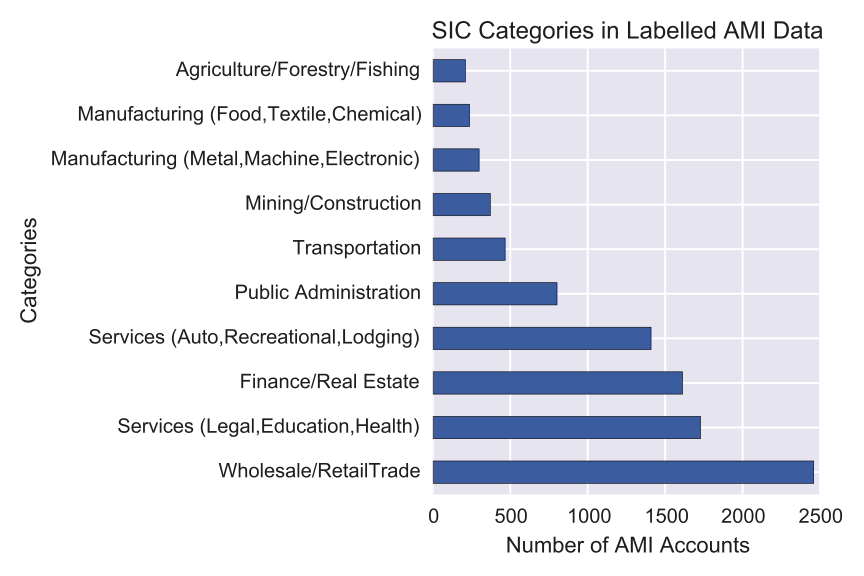
\includegraphics[width=0.84\columnwidth]{figures/measures/measures}
\caption{{Building Type Classification of the Labeled AMI Accounts
\label{fig:buildingtypeclass}%
}}
\end{center}
\end{figure}

Four classification models are then created to predict the general SIC Category of each account:
\begin{itemize}
\item Baseline model - using the distributions of the input samples to guess the category
\item Non-Temporal Features Model -- using non-temporal features containing monthly data and zip code/location information
\item Temporal Features -- using the new features generated from the AMI data
\item Combined Features -- using all the features, temporal and non-temporal
\end{itemize}

Once again a random forest model was implemented using Python's Scikit-Learn library. The models were executed an out-of-bag error to calculate mean model accuracy of a multi-label classification. Figure \ref{fig:modelimprovement_ami} illustrates the results of the models with respect to percent mean accuracy improvement over the baseline.


\begin{figure}[ht!]
\begin{center}
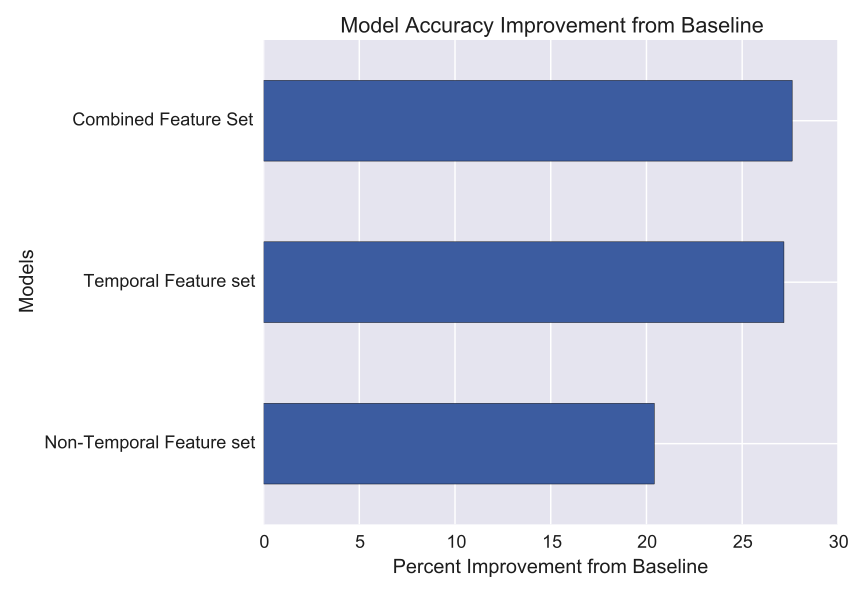
\includegraphics[width=0.84\columnwidth]{figures/classificationimprovement_AMI/classificationimprovement_AMI}
\caption{{Mean Model Accuracy Improvement from Baseline
\label{fig:modelimprovement_ami}%
}}
\end{center}
\end{figure}

The baseline model correctly predicts the labels with a 18.1\% accuracy, while the features influenced models were 38.5\% for Non-Temporal, 45.3\% for the Temporal and 45.7\% for the combined model.  The baseline model represents common practice in which a class is chosen based on the probability distribution of that class occurring in the labeled dataset. The combined feature set more than doubles the probability of predicting this piece of meta-data.

Mean accuracy of multi-label classification models as done in this analysis is a harsh metric as it forces the model to make a single choice for labeling each sample. In practice, it is not desired for a model that completely makes this decision; but instead to simply want the model to inform what the probability that a sample fits within a class. For example, there could be 45\% chance an unlabeled account is an office, a 35\% chance it is a school and 20\% chance it is a grocery store. The reason to choose mean model accuracy in this report it to communicate a simplified message of the techniques and the progress made thus far. The fact that the overall classification model accuracy is around 40-60\% for a classification model with ten classes is not discouraging. It is the improvement in mean accuracy from baselines that is the focus and this has been demonstrated so far in the project. 
%Additionally, there are other classification metrics including precision, recall, and F-Score that we have left out from this report that can be used to determine model usefulness. 

It can also be seen in detail how the model predicts the classes for each by creating and analyzing a classification confusion matrix. Figure \ref{fig:industry_classification} illustrates this matrix for the combined model. It is observed that two of the largest classes, Retail and Finance, have the highest accuracy rates at over 55-60\% with several other categories being misclassified within them.  This issue is common with imbalanced classification models and further feature development would improve the model by better characterizing the difference between each class.


\begin{figure}[ht!]
\begin{center}
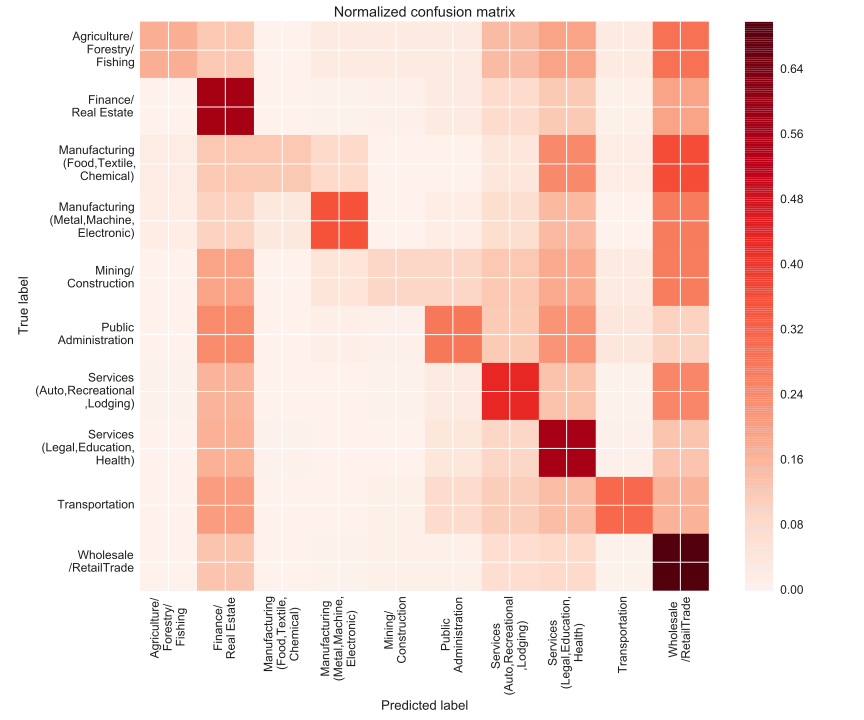
\includegraphics[width=1\columnwidth]{figures/classificationconfusionmatrix/classificationconfusionmatrix}
\caption{{Classification error matrix for prediction of standard industry class (SIC) using a random forest model
\label{fig:industry_classification}%
}}
\end{center}
\end{figure}

\section{Energy Efficiency Measure Implementation Success Prediction}
\label{sec:measuresuccess}

The next example of using the temporal features is predicting the success of future measure implementation events using the past data. For this proof-of-concept, Pre and Post-measure implementation data are utilized from close to 1,600 buildings that had one or more measures implemented. The difference in mean daily consumption before an after the measure implementation is calculated to achieve a rough indication of measure success. The measures into three classifications is divided according to where the difference in daily consumption for each account fits in the range of values. In this analysis, the accounts in the lowest 33\% were considered "Poor", while the 66\% percentile were "Average" and the top 33\% are considered "Good". Simple difference in mean daily consumption is not a perfect metric for success, as it is not normalized for weather or occupancy changes; although it is adequate for this step as we are already arbitrarily choosing the thresholds for class difference anyway and are looking for a simple metric at this point. 

% We recognize that improvement of this success metric is an obvious improvement in the methodology that can be pursued going forward.

Figure \ref{fig:measurecatbreakdown} illustrates a breakdown of the measure categories within the tested dataset. 
%This data is from the KITT platform and these are the accounts that have had only one month of measure implementation from each category implemented in the targeted time range.

\begin{figure}[ht!]
\begin{center}
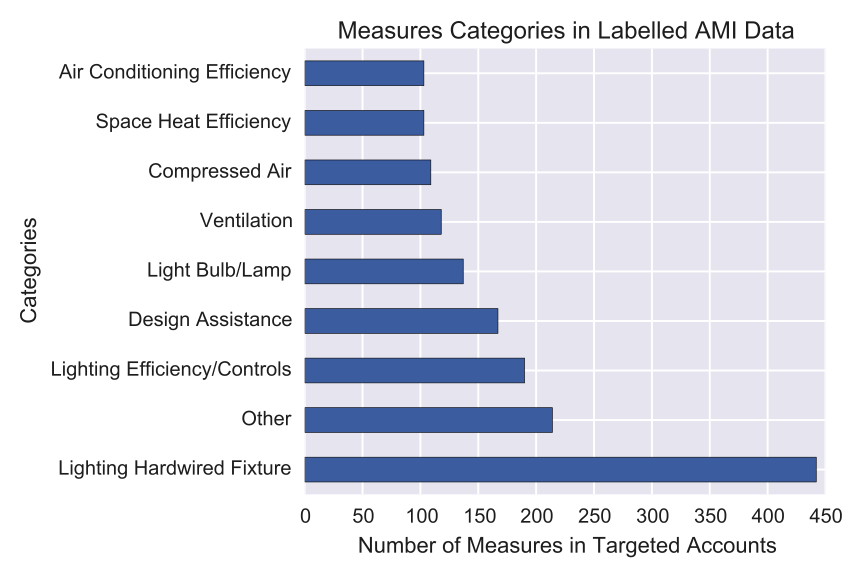
\includegraphics[width=0.7\columnwidth]{figures/measures_ami/measures_ami}
\caption{{Breakdown of Measure Categories included in the Dataset
\label{fig:measurecatbreakdown}%
}}
\end{center}
\end{figure}

A Random Forest algorithm was implemented to use the temporal features to predict the class of potential measure success (Good, Average or Poor). Figure \ref{fig:measurimp_classification} illustrates the classification error matrix for this model. 

\begin{figure}[ht!]
\begin{center}
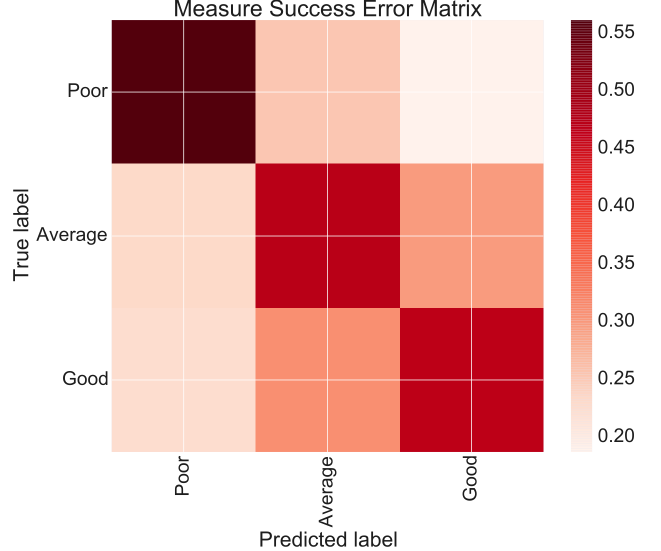
\includegraphics[width=0.7\columnwidth]{figures/measurespredictionmatrix/measurespredictionmatrix}
\caption{{Classification error matrix for prediction of measure implementation success using a random forest model
\label{fig:measurimp_classification}%
}}
\end{center}
\end{figure}

The baseline model with this data is able to predict the success within this set of classification at 32.8\% accuracy, while the model based on temporal features achieved 51.1\% accuracy. The more important aspect to pay attention to is that the misclassification rate between "Good" and "Poor" is less than 20\% -- a promising fact that motivates further investigation using the existing temporal data-set.

\section{Discussion}
\label{sec:scalabilitydiscussion}

This section discusses the creation of additional information about smart meter by extracting characteristics from the high-frequency time-series measurements. Based on a classification test using almost 9,600 labeled smart meter accounts, the accuracy of predicting building type is improved (based on SIC 1-Digit category) by over 27\% over a conventional baseline. 

Data about energy efficiency measures implementation and classified almost 1,600 accounts was aggregated into Good, Average, and Poor performing classes according to pre and post-measure consumption. A classification model is developed that improves the ability to predict measure implementation class success by 18\% over a baseline. Additionally, there was only a 20\% error rate in differentiating between Good and Poor performing measures.

The biggest opportunity ahead is to characterize missing meta-data and predict measure implementation success for future projects. Much work is also yet to be done to improve the models and input information to bring the overall prediction accuracies higher in absolute terms. Model prediction can also be improved incrementally as the AMI and measures implementation data are better integrated. 